% Created by tikzDevice version 0.9 on 2016-02-03 14:09:58
% !TEX encoding = UTF-8 Unicode
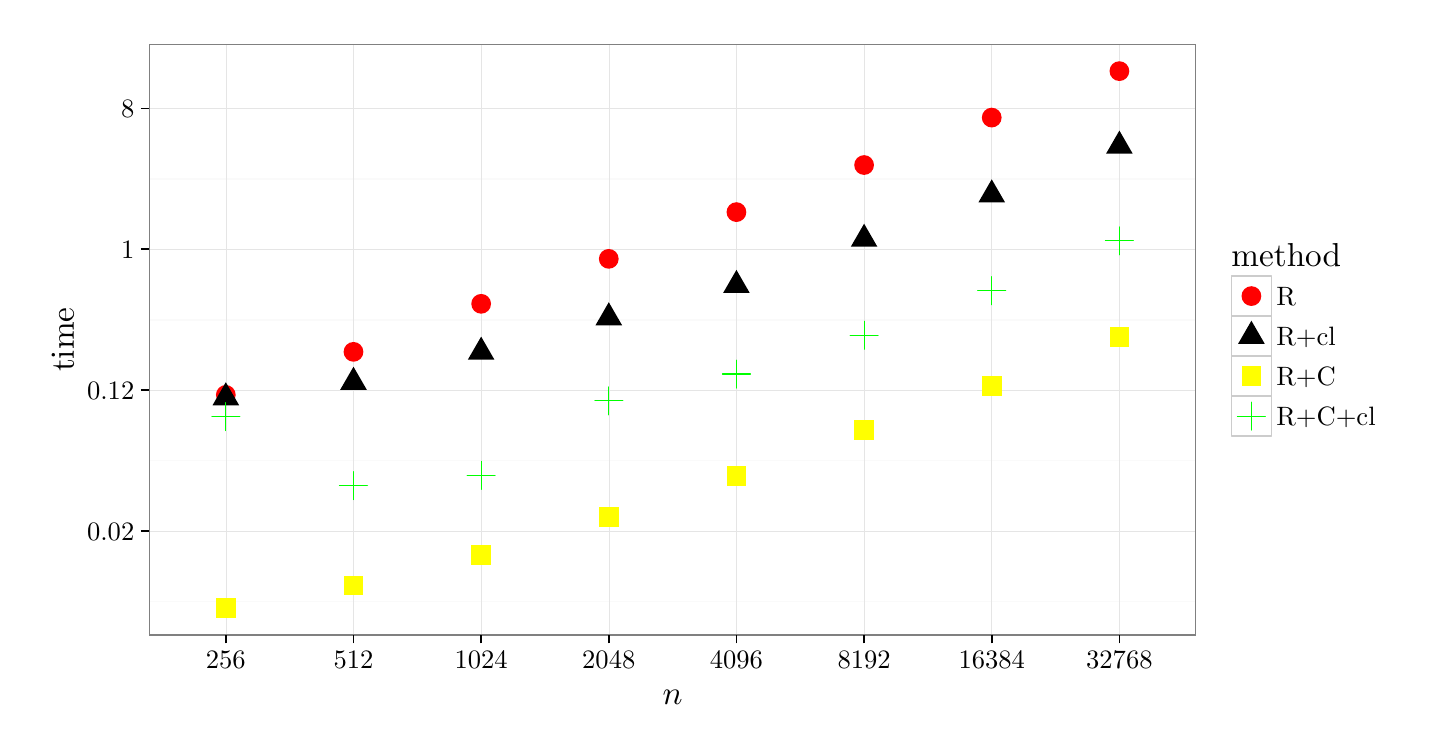
\begin{tikzpicture}[x=1pt,y=1pt]
\definecolor{fillColor}{RGB}{255,255,255}
\path[use as bounding box,fill=fillColor,fill opacity=0.00] (0,0) rectangle (505.89,252.94);
\begin{scope}
\path[clip] (  0.00,  0.00) rectangle (505.89,252.94);
\definecolor{drawColor}{RGB}{255,255,255}
\definecolor{fillColor}{RGB}{255,255,255}

\path[draw=drawColor,line width= 0.6pt,line join=round,line cap=round,fill=fillColor] (  0.00,  0.00) rectangle (505.89,252.95);
\end{scope}
\begin{scope}
\path[clip] ( 43.93, 33.48) rectangle (422.16,246.94);
\definecolor{fillColor}{RGB}{255,255,255}

\path[fill=fillColor] ( 43.93, 33.48) rectangle (422.16,246.94);
\definecolor{drawColor}{gray}{0.98}

\path[draw=drawColor,line width= 0.6pt,line join=round] ( 43.93, 45.62) --
	(422.16, 45.62);

\path[draw=drawColor,line width= 0.6pt,line join=round] ( 43.93, 96.52) --
	(422.16, 96.52);

\path[draw=drawColor,line width= 0.6pt,line join=round] ( 43.93,147.41) --
	(422.16,147.41);

\path[draw=drawColor,line width= 0.6pt,line join=round] ( 43.93,198.31) --
	(422.16,198.31);
\definecolor{drawColor}{gray}{0.90}

\path[draw=drawColor,line width= 0.2pt,line join=round] ( 43.93, 71.07) --
	(422.16, 71.07);

\path[draw=drawColor,line width= 0.2pt,line join=round] ( 43.93,121.97) --
	(422.16,121.97);

\path[draw=drawColor,line width= 0.2pt,line join=round] ( 43.93,172.86) --
	(422.16,172.86);

\path[draw=drawColor,line width= 0.2pt,line join=round] ( 43.93,223.76) --
	(422.16,223.76);

\path[draw=drawColor,line width= 0.2pt,line join=round] ( 71.60, 33.48) --
	( 71.60,246.94);

\path[draw=drawColor,line width= 0.2pt,line join=round] (117.73, 33.48) --
	(117.73,246.94);

\path[draw=drawColor,line width= 0.2pt,line join=round] (163.86, 33.48) --
	(163.86,246.94);

\path[draw=drawColor,line width= 0.2pt,line join=round] (209.98, 33.48) --
	(209.98,246.94);

\path[draw=drawColor,line width= 0.2pt,line join=round] (256.11, 33.48) --
	(256.11,246.94);

\path[draw=drawColor,line width= 0.2pt,line join=round] (302.24, 33.48) --
	(302.24,246.94);

\path[draw=drawColor,line width= 0.2pt,line join=round] (348.36, 33.48) --
	(348.36,246.94);

\path[draw=drawColor,line width= 0.2pt,line join=round] (394.49, 33.48) --
	(394.49,246.94);
\definecolor{fillColor}{RGB}{255,0,0}

\path[fill=fillColor] ( 71.60,120.24) circle (  3.57);

\path[fill=fillColor] (117.73,135.80) circle (  3.57);

\path[fill=fillColor] (163.86,153.15) circle (  3.57);

\path[fill=fillColor] (209.98,169.40) circle (  3.57);

\path[fill=fillColor] (256.11,186.29) circle (  3.57);

\path[fill=fillColor] (302.24,203.30) circle (  3.57);

\path[fill=fillColor] (348.36,220.45) circle (  3.57);

\path[fill=fillColor] (394.49,237.24) circle (  3.57);
\definecolor{fillColor}{RGB}{0,0,0}

\path[fill=fillColor] ( 71.60,124.83) --
	( 76.41,116.50) --
	( 66.80,116.50) --
	cycle;

\path[fill=fillColor] (117.73,130.42) --
	(122.54,122.09) --
	(112.92,122.09) --
	cycle;

\path[fill=fillColor] (163.86,141.30) --
	(168.66,132.97) --
	(159.05,132.97) --
	cycle;

\path[fill=fillColor] (209.98,153.73) --
	(214.79,145.40) --
	(205.18,145.40) --
	cycle;

\path[fill=fillColor] (256.11,165.41) --
	(260.91,157.09) --
	(251.30,157.09) --
	cycle;

\path[fill=fillColor] (302.24,182.11) --
	(307.04,173.78) --
	(297.43,173.78) --
	cycle;

\path[fill=fillColor] (348.36,198.14) --
	(353.17,189.82) --
	(343.56,189.82) --
	cycle;

\path[fill=fillColor] (394.49,215.76) --
	(399.29,207.43) --
	(389.68,207.43) --
	cycle;
\definecolor{fillColor}{RGB}{255,255,0}

\path[fill=fillColor] ( 68.03, 39.61) --
	( 75.17, 39.61) --
	( 75.17, 46.75) --
	( 68.03, 46.75) --
	cycle;

\path[fill=fillColor] (114.16, 47.85) --
	(121.30, 47.85) --
	(121.30, 54.98) --
	(114.16, 54.98) --
	cycle;

\path[fill=fillColor] (160.29, 58.91) --
	(167.42, 58.91) --
	(167.42, 66.05) --
	(160.29, 66.05) --
	cycle;

\path[fill=fillColor] (206.41, 72.61) --
	(213.55, 72.61) --
	(213.55, 79.74) --
	(206.41, 79.74) --
	cycle;

\path[fill=fillColor] (252.54, 87.24) --
	(259.68, 87.24) --
	(259.68, 94.38) --
	(252.54, 94.38) --
	cycle;

\path[fill=fillColor] (298.67,104.12) --
	(305.80,104.12) --
	(305.80,111.25) --
	(298.67,111.25) --
	cycle;

\path[fill=fillColor] (344.79,119.87) --
	(351.93,119.87) --
	(351.93,127.01) --
	(344.79,127.01) --
	cycle;

\path[fill=fillColor] (390.92,137.47) --
	(398.06,137.47) --
	(398.06,144.61) --
	(390.92,144.61) --
	cycle;
\definecolor{drawColor}{RGB}{0,255,0}

\path[draw=drawColor,line width= 0.4pt,line join=round,line cap=round] ( 66.56,112.38) -- ( 76.65,112.38);

\path[draw=drawColor,line width= 0.4pt,line join=round,line cap=round] ( 71.60,107.33) -- ( 71.60,117.43);

\path[draw=drawColor,line width= 0.4pt,line join=round,line cap=round] (112.68, 87.44) -- (122.78, 87.44);

\path[draw=drawColor,line width= 0.4pt,line join=round,line cap=round] (117.73, 82.39) -- (117.73, 92.49);

\path[draw=drawColor,line width= 0.4pt,line join=round,line cap=round] (158.81, 91.16) -- (168.90, 91.16);

\path[draw=drawColor,line width= 0.4pt,line join=round,line cap=round] (163.86, 86.11) -- (163.86, 96.20);

\path[draw=drawColor,line width= 0.4pt,line join=round,line cap=round] (204.94,118.10) -- (215.03,118.10);

\path[draw=drawColor,line width= 0.4pt,line join=round,line cap=round] (209.98,113.06) -- (209.98,123.15);

\path[draw=drawColor,line width= 0.4pt,line join=round,line cap=round] (251.06,127.78) -- (261.16,127.78);

\path[draw=drawColor,line width= 0.4pt,line join=round,line cap=round] (256.11,122.73) -- (256.11,132.82);

\path[draw=drawColor,line width= 0.4pt,line join=round,line cap=round] (297.19,141.79) -- (307.28,141.79);

\path[draw=drawColor,line width= 0.4pt,line join=round,line cap=round] (302.24,136.75) -- (302.24,146.84);

\path[draw=drawColor,line width= 0.4pt,line join=round,line cap=round] (343.31,157.88) -- (353.41,157.88);

\path[draw=drawColor,line width= 0.4pt,line join=round,line cap=round] (348.36,152.83) -- (348.36,162.93);

\path[draw=drawColor,line width= 0.4pt,line join=round,line cap=round] (389.44,175.93) -- (399.53,175.93);

\path[draw=drawColor,line width= 0.4pt,line join=round,line cap=round] (394.49,170.89) -- (394.49,180.98);
\definecolor{drawColor}{gray}{0.50}

\path[draw=drawColor,line width= 0.6pt,line join=round,line cap=round] ( 43.93, 33.48) rectangle (422.16,246.94);
\end{scope}
\begin{scope}
\path[clip] (  0.00,  0.00) rectangle (505.89,252.94);
\definecolor{drawColor}{RGB}{0,0,0}

\node[text=drawColor,anchor=base east,inner sep=0pt, outer sep=0pt, scale=  0.96] at ( 38.53, 67.76) {0.02};

\node[text=drawColor,anchor=base east,inner sep=0pt, outer sep=0pt, scale=  0.96] at ( 38.53,118.66) {0.12};

\node[text=drawColor,anchor=base east,inner sep=0pt, outer sep=0pt, scale=  0.96] at ( 38.53,169.56) {1};

\node[text=drawColor,anchor=base east,inner sep=0pt, outer sep=0pt, scale=  0.96] at ( 38.53,220.45) {8};
\end{scope}
\begin{scope}
\path[clip] (  0.00,  0.00) rectangle (505.89,252.94);
\definecolor{drawColor}{RGB}{0,0,0}

\path[draw=drawColor,line width= 0.6pt,line join=round] ( 40.93, 71.07) --
	( 43.93, 71.07);

\path[draw=drawColor,line width= 0.6pt,line join=round] ( 40.93,121.97) --
	( 43.93,121.97);

\path[draw=drawColor,line width= 0.6pt,line join=round] ( 40.93,172.86) --
	( 43.93,172.86);

\path[draw=drawColor,line width= 0.6pt,line join=round] ( 40.93,223.76) --
	( 43.93,223.76);
\end{scope}
\begin{scope}
\path[clip] (  0.00,  0.00) rectangle (505.89,252.94);
\definecolor{drawColor}{RGB}{0,0,0}

\path[draw=drawColor,line width= 0.6pt,line join=round] ( 71.60, 30.48) --
	( 71.60, 33.48);

\path[draw=drawColor,line width= 0.6pt,line join=round] (117.73, 30.48) --
	(117.73, 33.48);

\path[draw=drawColor,line width= 0.6pt,line join=round] (163.86, 30.48) --
	(163.86, 33.48);

\path[draw=drawColor,line width= 0.6pt,line join=round] (209.98, 30.48) --
	(209.98, 33.48);

\path[draw=drawColor,line width= 0.6pt,line join=round] (256.11, 30.48) --
	(256.11, 33.48);

\path[draw=drawColor,line width= 0.6pt,line join=round] (302.24, 30.48) --
	(302.24, 33.48);

\path[draw=drawColor,line width= 0.6pt,line join=round] (348.36, 30.48) --
	(348.36, 33.48);

\path[draw=drawColor,line width= 0.6pt,line join=round] (394.49, 30.48) --
	(394.49, 33.48);
\end{scope}
\begin{scope}
\path[clip] (  0.00,  0.00) rectangle (505.89,252.94);
\definecolor{drawColor}{RGB}{0,0,0}

\node[text=drawColor,anchor=base,inner sep=0pt, outer sep=0pt, scale=  0.96] at ( 71.60, 21.46) {256};

\node[text=drawColor,anchor=base,inner sep=0pt, outer sep=0pt, scale=  0.96] at (117.73, 21.46) {512};

\node[text=drawColor,anchor=base,inner sep=0pt, outer sep=0pt, scale=  0.96] at (163.86, 21.46) {1024};

\node[text=drawColor,anchor=base,inner sep=0pt, outer sep=0pt, scale=  0.96] at (209.98, 21.46) {2048};

\node[text=drawColor,anchor=base,inner sep=0pt, outer sep=0pt, scale=  0.96] at (256.11, 21.46) {4096};

\node[text=drawColor,anchor=base,inner sep=0pt, outer sep=0pt, scale=  0.96] at (302.24, 21.46) {8192};

\node[text=drawColor,anchor=base,inner sep=0pt, outer sep=0pt, scale=  0.96] at (348.36, 21.46) {16384};

\node[text=drawColor,anchor=base,inner sep=0pt, outer sep=0pt, scale=  0.96] at (394.49, 21.46) {32768};
\end{scope}
\begin{scope}
\path[clip] (  0.00,  0.00) rectangle (505.89,252.94);
\definecolor{drawColor}{RGB}{0,0,0}

\node[text=drawColor,anchor=base,inner sep=0pt, outer sep=0pt, scale=  1.20] at (233.05,  8.40) {$n$};
\end{scope}
\begin{scope}
\path[clip] (  0.00,  0.00) rectangle (505.89,252.94);
\definecolor{drawColor}{RGB}{0,0,0}

\node[text=drawColor,rotate= 90.00,anchor=base,inner sep=0pt, outer sep=0pt, scale=  1.20] at ( 16.66,140.21) {time};
\end{scope}
\begin{scope}
\path[clip] (  0.00,  0.00) rectangle (505.89,252.94);
\definecolor{fillColor}{RGB}{255,255,255}

\path[fill=fillColor] (430.70,101.10) rectangle (491.35,179.33);
\end{scope}
\begin{scope}
\path[clip] (  0.00,  0.00) rectangle (505.89,252.94);
\definecolor{drawColor}{RGB}{0,0,0}

\node[text=drawColor,anchor=base west,inner sep=0pt, outer sep=0pt, scale=  1.20] at (434.97,166.79) {method};
\end{scope}
\begin{scope}
\path[clip] (  0.00,  0.00) rectangle (505.89,252.94);
\definecolor{drawColor}{gray}{0.80}
\definecolor{fillColor}{RGB}{255,255,255}

\path[draw=drawColor,line width= 0.6pt,line join=round,line cap=round,fill=fillColor] (434.97,148.73) rectangle (449.42,163.18);
\end{scope}
\begin{scope}
\path[clip] (  0.00,  0.00) rectangle (505.89,252.94);
\definecolor{fillColor}{RGB}{255,0,0}

\path[fill=fillColor] (442.19,155.95) circle (  3.57);
\end{scope}
\begin{scope}
\path[clip] (  0.00,  0.00) rectangle (505.89,252.94);
\definecolor{drawColor}{gray}{0.80}
\definecolor{fillColor}{RGB}{255,255,255}

\path[draw=drawColor,line width= 0.6pt,line join=round,line cap=round,fill=fillColor] (434.97,134.27) rectangle (449.42,148.73);
\end{scope}
\begin{scope}
\path[clip] (  0.00,  0.00) rectangle (505.89,252.94);
\definecolor{fillColor}{RGB}{0,0,0}

\path[fill=fillColor] (442.19,147.05) --
	(447.00,138.72) --
	(437.39,138.72) --
	cycle;
\end{scope}
\begin{scope}
\path[clip] (  0.00,  0.00) rectangle (505.89,252.94);
\definecolor{drawColor}{gray}{0.80}
\definecolor{fillColor}{RGB}{255,255,255}

\path[draw=drawColor,line width= 0.6pt,line join=round,line cap=round,fill=fillColor] (434.97,119.82) rectangle (449.42,134.27);
\end{scope}
\begin{scope}
\path[clip] (  0.00,  0.00) rectangle (505.89,252.94);
\definecolor{fillColor}{RGB}{255,255,0}

\path[fill=fillColor] (438.63,123.48) --
	(445.76,123.48) --
	(445.76,130.61) --
	(438.63,130.61) --
	cycle;
\end{scope}
\begin{scope}
\path[clip] (  0.00,  0.00) rectangle (505.89,252.94);
\definecolor{drawColor}{gray}{0.80}
\definecolor{fillColor}{RGB}{255,255,255}

\path[draw=drawColor,line width= 0.6pt,line join=round,line cap=round,fill=fillColor] (434.97,105.36) rectangle (449.42,119.82);
\end{scope}
\begin{scope}
\path[clip] (  0.00,  0.00) rectangle (505.89,252.94);
\definecolor{drawColor}{RGB}{0,255,0}

\path[draw=drawColor,line width= 0.4pt,line join=round,line cap=round] (437.15,112.59) -- (447.24,112.59);

\path[draw=drawColor,line width= 0.4pt,line join=round,line cap=round] (442.19,107.54) -- (442.19,117.64);
\end{scope}
\begin{scope}
\path[clip] (  0.00,  0.00) rectangle (505.89,252.94);
\definecolor{drawColor}{RGB}{0,0,0}

\node[text=drawColor,anchor=base west,inner sep=0pt, outer sep=0pt, scale=  0.96] at (451.23,152.65) {R};
\end{scope}
\begin{scope}
\path[clip] (  0.00,  0.00) rectangle (505.89,252.94);
\definecolor{drawColor}{RGB}{0,0,0}

\node[text=drawColor,anchor=base west,inner sep=0pt, outer sep=0pt, scale=  0.96] at (451.23,138.19) {R+cl};
\end{scope}
\begin{scope}
\path[clip] (  0.00,  0.00) rectangle (505.89,252.94);
\definecolor{drawColor}{RGB}{0,0,0}

\node[text=drawColor,anchor=base west,inner sep=0pt, outer sep=0pt, scale=  0.96] at (451.23,123.74) {R+C};
\end{scope}
\begin{scope}
\path[clip] (  0.00,  0.00) rectangle (505.89,252.94);
\definecolor{drawColor}{RGB}{0,0,0}

\node[text=drawColor,anchor=base west,inner sep=0pt, outer sep=0pt, scale=  0.96] at (451.23,109.28) {R+C+cl};
\end{scope}
\end{tikzpicture}
